\documentclass[
    iict, % Saisir le nom de l'institut rattaché
    il, % Saisir le nom de l'orientation
    %confidential, % Décommentez si le travail est confidentiel
]{heig-tb}

\usepackage[nooldvoltagedirection,european,americaninductors]{circuitikz}
\usepackage{lscape}
\signature{mbernasconi.svg} % Remplacer par votre propre signature vectorielle.

\makenomenclature
\makenoidxglossaries
\makeindex

\addbibresource{bibliography.bib}

\usepackage{etoolbox}
\renewcommand\nomgroup[1]{%
  \item[\bfseries
              \ifstrequal{#1}{A}{Constantes physiques}{%
                \ifstrequal{#1}{B}{Groupes}{%
                  \ifstrequal{#1}{C}{Autres Symboles}{}}}%
        ]}

\newcommand{\nomunit}[1]{%
  \renewcommand{\nomentryend}{\hspace*{\fill}#1}}

\nomenclature[A, 02]{\(c\)}{\href{https://physics.nist.gov/cgi-bin/cuu/Value?c}
  {Vitesse de la lumière dans le vide}
  \nomunit{\SI{299792458}{\meter\per\second}}}

\nomenclature[A, 03]{\(h\)}{\href{https://physics.nist.gov/cgi-bin/cuu/Value?h}
  {Constante de Planck}
  \nomunit{\SI[group-digits=false]{6.62607015e-34}{\joule\per\hertz}}}

\nomenclature[A, 01]{\(G\)}{\href{https://physics.nist.gov/cgi-bin/cuu/Value?bg}
  {Constante de gravitation universelle}
  \nomunit{\SI[group-digits=false]{6.67430e-11}{\meter\cubed\per\kilogram\per\second\squared}}}

\nomenclature[B, 03]{\(\mathbb{R}\)}{Nombres réels}
\nomenclature[B, 02]{\(\mathbb{C}\)}{Nombres complexes}
\nomenclature[B, 01]{\(\mathbb{H}\)}{Quaternions}

\nomenclature[C]{\(V\)}{Volume constant}
\nomenclature[C]{\(\rho\)}{Indice de frottement sec}

\newacronym{gcd}{GCD}{Plus grand diviseur commun}
\newacronym{lcm}{LCM}{Plus petit multiple commun}

\newglossaryentry{heig-vd}{
    name=HEIG-VD,
    description={Haute École d'Ingénierie et de Gestion du canton de Vaud}
}
\newglossaryentry{hes-so}{
    name=HES-SO,
    description={Haute École Supérieure de Suisse Occidentale}
}
\newglossaryentry{latex}{
    name=latex,
    description={Un langage et un système de composition de documents}
}
\newglossaryentry{maths}{
    name=mathematics,
    description={Les mathematiques sont ce que les mathématiciens fonts}
}
% Auteur du document (étudiant-e) en projet de Bachelor
\author{Nelson Jeanrenaud}

% Activer l'option pour l'accord du féminin dans le texte
\genre{male}

% Titre de votre travail de Bachelor
\title{Machine Learning pour prendre la décision d'un arrêt au stand en Formule 1}

% Le sous titre est optionnel
\subtitle{Rapport Intermédiaire Travail de Bachelor}

% Nom du professeur responsable
\teacher {Pena Carlos Andrés (HEIG-VD)}

% Mettre à jour avec la date de rendu du travail
\date{\today}

% Numéro de TB
\thesis{7212}



\surroundwithmdframed{minted}

%% Début du document
\begin{document}
\selectlanguage{french}
\maketitle
\frontmatter
\clearemptydoublepage

%% Requis par les dispositions générales des travaux de Bachelor
\preamble
\authentification

%% Résumé / Résumé publiable / Version abrégée
\begin{abstract}
    % Francais
L'objectif d'une course automobile est de parcourir un nombre de tours sur un circuit le plus
rapidement possible. De plus, dans de nombreuses catégories, les voitures peuvent s'arrêter au stand pour changer de pneus et/ ou se réapprovisionner en carburant.
La dégradation des pneus et le poids supplémentaire dû à la charge de carburant ont un impact majeur sur les temps au tour d'une voiture.
Décider quand et combien de fois rentrer dans les stands est donc crucial pour les écuries. À cela vienne s'ajouter les notions de neutralisation de la course pour cause d'incident.

Établir la stratégie optimale est un enjeu majeur pour les équipes de course. Il est donc nécessaire de développer un système d'analyse de données et de prédiction pour aider les écuries à prendre les meilleures décisions stratégiques pendant la course.
Ce système devra prendre en compte les données de la voiture, les performances des pneus et les conditions de la piste pour fournir des recommandations en temps réel aux équipes de course.

Dans ce travail, nous tentons de créer un tel système pour le championnat du monde de Formule 1.
Pour ce faire, nous entraînons des modèles de Machine Learning sur des données historiques de la dernière ère de la formule 1.

Un set de données a été établi à partir des données transmises par la Formule 1 pendant les courses.
Ces données ont été préparées de manière à former un ensemble complet et cohérent, permettant d'entraîner des modèles

Après l'expérimentation avec des réseaux de neurones et des réseaux de neurones récurrents,
nous avons réussi à développer des modèles capables de capturer les relations entre la stratégie de course et les données de la voiture.

Pour améliorer le système, nous pourrions inclure les facteurs météorologiques, développer une simulation de course pour améliorer la précision des prédictions
et tester l'apprentissage par renforcement pour développer des stratégies novatrices.
\end{abstract}

%% Sommaire et tables
\clearemptydoublepage
{
    \tableofcontents
    \let\cleardoublepage\clearpage
    \listoffigures
    \let\cleardoublepage\clearpage
    \listoftables
    %    \let\cleardoublepage\clearpage
    %    \listoflistings
}

\printnomenclature
\clearemptydoublepage
\pagenumbering{arabic}

%% Contenu
\mainmatter
\chapter{Introduction}
\section{Objectifs}
Les objectifs de ce projet sont de développer un système de prédiction de stratégie de course en temps réel pour les équipes de course, basé sur l'analyse des données de la voiture et des conditions de la piste, et de fournir des recommandations pour optimiser les temps de tour et les arrêts aux stands.
\subsection{Objectifs fondamentaux}
\begin{itemize}
    \item Implémenter un pipeline de traitement et d’analyse de données avec des algorithmes de Machine Learning pour recommander l’entrée au stand d’une voiture en fonction de la situation de course.
    \item Établir un dataset adéquat à l’entrainement d’un tel modèle à partir de multiples sources de données brutes.
    \item Fournir des prédictions réalistes et interprétables par les experts métiers.
    \item Le système est réactif et permet des prédictions rapides (moins de 30 secondes).
\end{itemize}
\subsection{Objectifs optionnels}
\begin{itemize}
    \item Développer une interface utilisateur pour facilement accéder aux recommandations stratégiques.
    \item Étendre le modèle pour les conditions météorologiques incertaines comme les chutes de pluie.
\end{itemize}

\section{Principe de la stratégie en Formule 1}
L'objectif fondamental de la stratégie est de minimiser le temps que l'on prend pour finir tous les tours de course.
En formule 1, les écuries doivent choisir entre 3 composés de pneumatique à utiliser.
Ces composés nommés tendres, mediums et durs performent différemment le long de la course, les plus tendres offrant une meilleure adhérence, mais s'usant plus rapidement.

Pour illustrer cette section on a simulé en python une course très simplifiée. La simulation considère que la voiture est seule sur la piste,
qu'il n'y a pas de variation dans la performance du pilote ou dans l'état du circuit.
La course est discrétisée en $N$ tours où chaque temps au tour $t_{tour}$ est défini comme montré dans l'équation \ref{eq:tour} :

\begin{equation} \label{eq:tour}
    \begin{split}
        t_{tour}=t_{optimal} + t_{carburant} + t_{pneu}
    \end{split}
\end{equation}

$t_{optimal}$ est le temps optimal que la voiture peut faire sur le circuit dans les meilleures conditions.
$t_{carburant}$ est le temps perdu en raison du poids du carburant embarqué. Au fil de la course ce temps s'amoindrit lorsque que
le carburant est consommé. $t_{carburant}$ est calculé comme l'équation \ref{eq:carburant}.
Où $t_{penalite}$ est le temps au tour perdu par kg. Cette valeur dépend du circuit, mais est approximable à 0.03 seconde pour les circuits de longueur moyenne. \cite{royalAcademyOfEngineering} \cite{hurryUpAndWeight}
$p_{depart}$ est la quantité en kg de carburant au départ de la course, pour cette simulation, nous faisons l'hypothèse que la voiture commence avec le maximum de carburant autorisé, c'est-à-dire 110 kg.
$p_{consomme}$ est la quantité de carburant en kg qui est consommé en 1 tour de course, elle est calculée en estimant que la consommation de carburant est constante, soit $\frac{p_{depart}}{N}$.
$n$ est le nombre de tours parcourus jusqu'à maintenant.

\begin{equation} \label{eq:carburant}
    \begin{split}
        t_{carburant} = t_{penalite} * (p_{depart} - p_{consomme} * n)
    \end{split}
\end{equation}

$t_{pneu}$ est le temps perdu en raison de l'adhérence des pneumatiques, elle dépend du composé et de la dégradation du pneu. Le détail est donné dans l'équation \ref{eq:pneu},
elle approxime la dégradation des pneus par la formule de calcul des intérêts composés pour représenter la chute de performance que l'on peut observer avec les pneumatiques \cite{parttimeanalyst}.
$t_{per\textit{f}ormance}$ est le temps perdu comparé à la performance du pneu le plus tendre.
Le taux de dégradation du pneu par tour, exprimé en pourcentage par $d$ et le $\delta{d}$ l'augmentation de ce taux par tour.

\begin{equation} \label{eq:pneu}
    \begin{split}
        t_{pneu} = t_{per\textit{f}ormance} + d * (1 + \delta{d}) ^{(n - 1)}
    \end{split}
\end{equation}

La figure \ref{Comparaison de la dégradation} illustre l'influence de la dégradation sur la performance des différents composés de pneu utilisant
la simulation avec des paramètres trouvable dans la table \ref{Paramètres de la simulation} en annexe.
Les pneus tendres sont plus performant initialement avant de rapidement perdre en performance, le même phénomène se produit avec les mediums et les durs, mais après un plus grand laps de temps.
Cette différence en performance entre les composés dépend du circuit et est difficile à estimer précisément en amont de la course.

\fig[H, width=0.9\textwidth]{\label{Comparaison de la dégradation}Comparaison de la dégradation des différents composés de pneu}{compounds_comparison.svg}

Les temps au tour sont successivement additionnés pour obtenir la variable $t_{course}$, qui représente la durée totale d'une stratégie simulée comme présenté dans l'équation \ref{eq:course}.
\begin{equation} \label{eq:course}
    \begin{split}
        t_{course} = \sum_{i=1}^{N}{t_{tour}(i)}
    \end{split}
\end{equation}

On peut observer avec la figure \ref{Comparaison du temps de course} que sur une course de 70 tours utiliser les durs est la meilleure stratégie.
Cependant, le règlement de la Formule 1 oblige d'utiliser au minimum 2 composés différents par courses.
Il faut maintenant trouver le tour optimal où changer de pneumatique pour minimiser le temps de course total.
Une fois tous les paramètres établis, cela se ramène à un problème d'optimisation quadratique.
\fig[H, width=0.9\textwidth]{\label{Comparaison du temps de course}Comparaison du temps de course des différents composés de pneu}{compounds_total_race_time.svg}

La figure \ref{stratégies à 1 arrêt}, montre l'influence du tour d'arrêt sur le temps total de course.
On peut voir que pour notre course, la stratégie de commencer avec des tendres et les remplacer par des mediums après 20 à 30 tours est la plus rapide.

\fig[H, width=0.9\textwidth]{Comparaison du temps de course de différentes stratégies à 1 arrêt \label{stratégies à 1 arrêt}}{one_stop_strategies.svg}

Certains événements aléatoires comme les périodes de voiture de sécurité, impact grandement la stratégie. Une voiture de sécurité est déployée suite à un incident ou à la présence de débris sur la piste.
Dans cette situation, les voitures doivent rouler à vitesse réduite, ce qui réduit fortement le temps perdu pendant un arrêt au stand.
Cela est dû au fait que les voitures doivent toujours rouler à vitesse réduite dans la voie des stands même quand il n'y a pas de voiture de sécurité, la figure \ref{safety_car_1_stop} illustre ce phénomène.
Comparé à la course en figure \ref{stratégies à 1 arrêt} où la voiture de sécurité n'est pas déployée, il est plus intéressant de s'arrêter pendant la période de safety car même si les pneumatiques seront moins performant en fin de course.
\fig[H, width=0.9\textwidth]{Comparaison du temps de course de différentes stratégies à 1 arrêt avec une période de voiture de sécurité, en considérant que s'arrêter pendant cette période économise 10 secondes \label{safety_car_1_stop}}{one_stop_strategies_safety_car.svg}

D'autres éléments pas pris en compte dans cette simulation impactent la stratégie, notamment les autres voitures sur la piste.
Il est souvent intéressant de distancer suffisamment les voitures plus lentes derrière ou attendre qu'elles s'arrêtent avant de s'arrêter soit même pour éviter de perdre du temps à devoir les dépasser sur le circuit.
Une autre tactique est celle de l'undercut, utilisée quand un pilote à de la difficulté à dépasser une autre voiture. La technique consiste à s'arrêter plus tôt que prévu pour réduire l'écart avec la voiture poursuivie avec des pneus plus frais.
Si elle est bien exécutée l'adversaire se verra dépassé pendant qu'il effectue est dans la voie des stands.
C'est dans ce contexte qu'il serait intéressant de développer des méthodes de Machine Learning pour évaluer les décisions stratégiques.
\section{État de l'art}
Les modèles actuellement utilisés par les équipes de course pour établir leur stratégie de course sont évidemment confidentiels.
Néanmoins, il existe des articles publiés par des universités notamment “Application of Monte Carlo Methods to Consider Probabilistic Effects in a Race Simulation for Circuit Motorsport”. \cite{app10124229}
Cette étude présente une approche de simulation de course qui considère des éléments aléatoires tels que les accidents, les problèmes mécaniques
et les variations de performance des pilotes et des mécaniciens.

Un autre article du même institut, “Virtual Strategy Engineer: Using Artificial Neural Networks for Making Race Strategy Decisions in Circuit Motorsport”. \cite{app10217805}
se base sur ce simulateur pour entrainer des réseaux de neurones à la prise de décision stratégiques.
On peut noter des décisions intéressantes comme la division de la décision entre 2 modèles, le premier prends la décision de s’arrêter et l’autre choisis le composé de pneu à utiliser.
Ils ont développé des features intéressantes pour l'entrée de leur modèle notamment la catégorisation des circuits en 3 groupes selon le niveau de stress appliqué sur les pneumatiques,
la discrétisation de la position en "leader de la course ou non" et de la distance avec la voiture précédente en "Close ahead" qui est vrai si l'écart est inférieur à 1.5 seconde.
D'après leur étude, résoudre un problème d'optimisation de minimisation du temps de course dans un simulateur en amont permet de créer une feature
représentant le nombre d'arrêts au stand restant pour atteindre la stratégie optimale (1, 2 ou 3 arrêts).
Leurs résultats montre qu'une architecture feedforward considérant que le dernier tour de course n'arrive pas à modifier la probabilité d'un arrêt assez rapidement pour obtenir des résultats précis.
Ils ont expérimenté avec une architecture récurrente, considérant les 4 derniers tours obtenais de meilleurs résultats, mais faisait des erreurs difficilement compréhensibles.
L'architecture retenue est celle d'un réseau hybride avec un seul neurone long short-term memory. Leurs résultats sont présentés en table \ref{vse_results} et figure \ref{vse_ffnn}.

\begin{table}[H]
    \begin{center}
        \caption{\label{vse_results}Résultats de l'étude "Virtual Strategy Engineer: Using Artificial Neural Networks for Making Race Strategy Decisions in Circuit Motorsport"}
        \begin{tabular}{ll}
            Architecture & $F_1$ score \\ \hline
            Feedforward  & 0.35        \\
            Recurrent    & 0.9         \\
            Hybride      & 0.59
        \end{tabular}
    \end{center}
\end{table}

\begin{figure}[H]
    \begin{center}
        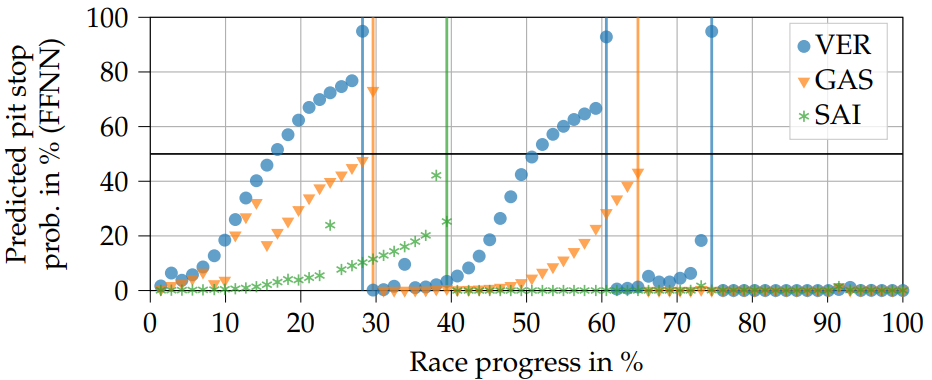
\includegraphics[width=0.7\textwidth]{assets/figures/vse_ffnn.png}
        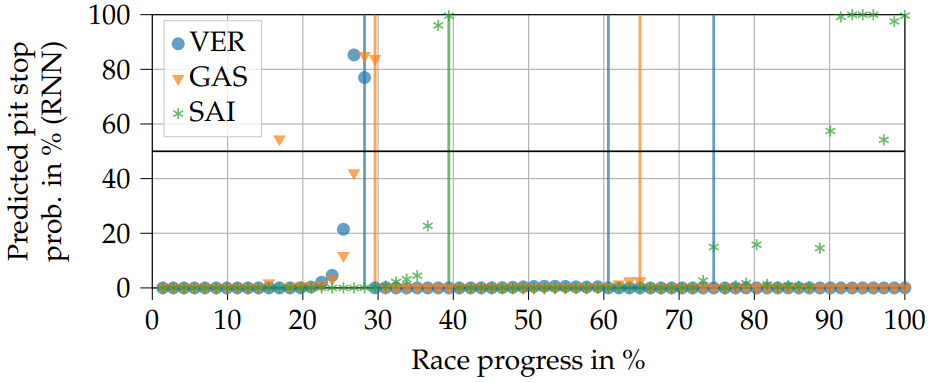
\includegraphics[width=0.7\textwidth]{assets/figures/vse_rnn.png}
        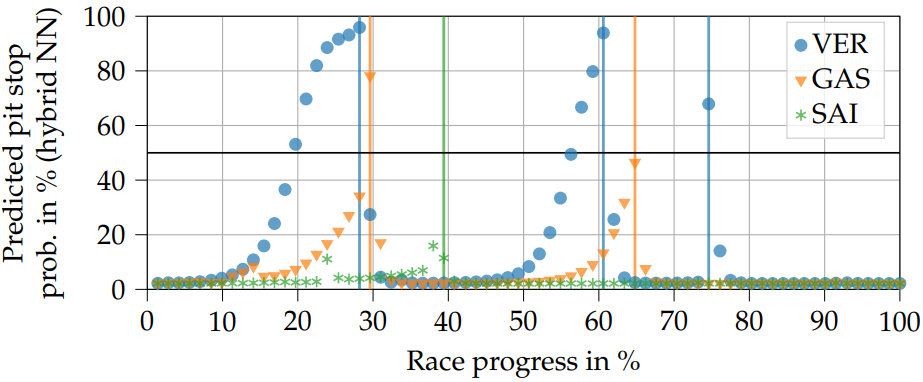
\includegraphics[width=0.7\textwidth]{assets/figures/vse_hnn.png}
        \caption{\label{vse_ffnn}Progression des probabilités d'arrêt au stand pour trois pilotes prédites par le réseau feed-forward, le réseau récurrent et le réseau hybride en utilisant des données du Grand Prix du Brésil 2019, figure repris du papier "Virtual Strategy Engineer: Using Artificial Neural Networks for Making Race Strategy Decisions in Circuit Motorsport"}
    \end{center}
\end{figure}

Les 2 travaux "Tire Changes, Fresh Air, and Yellow Flags: Challenges in Predictive Analytics for Professional Racing" \cite{doi:10.1089/big.2014.0018} et "Real-time decision making in motorsports : analytics for improving professional car race strategy"\cite{phdthesis}
sont des équivalences à notre problématique appliquée au monde de la NASCAR. La NASCAR est une course compétition américaine sur circuits ovales avec des voitures de série modifiées,
dans ce contexte, met davantage l'accent sur les courses en peloton, les dépassements sont plus fréquents et le ravitaillement en carburant est un facteur stratégique majeur.
Ils apportent cependant une formulation différente intéressante, la variable prédite par ses systèmes est le nombre de positions gagnées ou perdues à la suite d'une décision stratégique.

Finalement, on peut noter l'article “Formula-E race strategy development using distributed policy gradient reinforcement learning” de l'université de Cranfield \cite{LIU2021106781} qui utilise une approche de reinforcement learning pour établir une stratégie.
Cet article présente une méthode de développement de stratégies de course dans le contexte du championnat de Formule E, où les voitures ne changent pas de pneus et où la stratégie est davantage liée à l'économie de la batterie.
Cependant, bien que le contexte soit différent de celui proposé dans ce projet et que l'approche reinforcement learning nécessite une simulation précise, la méthode utilisée reste intéressante à noter.

\section{Méthodologie}
La méthodologie adoptée pour cette thèse comprendra les étapes suivantes. Tout d'abord, une analyse approfondie des données disponibles sera réalisée afin d'acquérir une connaissance approfondie de la problématique étudiée.
Ensuite, plusieurs formulations du problème, modèles et méthodes seront explorés à travers des expérimentations.
Les performances respectives de ces approches seront mesurées à l'aide de différentes métriques pour confirmer leur adéquation avec l'objectif fixé.
\chapter{Données}
Cette section est consacrée à l'étude des données disponibles sur les courses de Formule 1 et à la création d'un dataset adapté
à l'entrainement d'un modèle de Machine Learning.

\section{Données existantes}

Il existe 2 principales sources de données disponibles sur les courses de Formule 1.
La première est le dataset Ergast, qui est un projet open source qui répertorie des données sur les résultats des Grand Prix.
La seconde est la Formule 1 elle-même qui diffuse publiquement une certaine partie des données, dites "Live Timing",
qui correspondent aux données des capteurs des voitures.
Les données ont donc plusieurs temporalités :
\begin{itemize}
    \item les informations sur un weekend de courses (circuit, saison, etc.)
    \item les données pour un tour de course (temps au tour, gomme de pneu, etc.)
    \item les données des capteurs (vitesse, distance avec les autres voitures, etc.)
\end{itemize}

FastF1 est une librairie Python qui permet facilement d'accéder aux données de l'API Ergast et aux données officielle de la Formule 1 depuis 2018.
\fig[H, width=0.9\textwidth]{Diagramme en couches des données}{data_layers.svg}

La quantité entre les catégories de données que nous avons surnommés respectivement données de courses, données de tour et données de télémétrie
sont très différentes.

\fig[H, width=0.9\textwidth]{Nombre de données par courses, pour chaque catégorie de données}{nbSamples.svg}

\subsection{Données de courses}
Ces données donnent des informations sur le weekend de course et ne changent pas au cours de ce dernier.
La majorité des features de cette catégorie sont connues pendant la course et donc au moment de l'inférence.

\begin{table}[h]
    \begin{center}
        \caption{Liste d'exemple de features 'données de courses'}
        \begin{tabular}{l|l}
            Nom de la feature & Exemple de valeur \\ \hline
            season            & 2021              \\
            circuit           & Monaco            \\
            number of laps    & 78
        \end{tabular}
    \end{center}
\end{table}

Les autres features sont liées au résultat de la course et ne serais pas disponibles pendant la prédiction.
Mais elles pourraient être utilisées pendant l'entrainement pour par exemple pondérer plus fortement
les stratégies de voitures qui ont de meilleurs résultats.
\subsection{Données de tour}
L'API de la Formule 1 permet d'écouter un flux de données dit "Live Timing".
Ce flux contient différents canaux :
\begin{table}[H]
    \begin{center}
        \caption{Liste des différents canaux fournis dans le flux de données "Live Timing" \cite{fastf1documentation}}
        \begin{tabular}{l|l}
            Canal           & Description                                            \\ \hline
            LapNumber       & Numéro du tour en cours                                \\
            Driver          & Numéro identifiant du pilote                           \\
            LapTime         & Temps du tour précédent                                \\
            Stint           & Nombre de relais effectués                             \\
            TotalLaps       & Nombre total de tours effectués avec ce set de pneus   \\
            Compound        & Type de pneus utilisé                                  \\
            New             & Indique si le pneu a été neuf au moment de son montage \\
            TyresNotChanged & Signale les arrêts aux stands sans changement de pneus \\
            Time            & Temps écoulé depuis le début de la session             \\
            LapFlags        & Drapeaux survenus pendant le tour
        \end{tabular}
    \end{center}
\end{table}

À chaque instant, seulement certains canaux sont actifs. La librairie FastF1 effectue le travail de les agréger sur le parcours d'un tour. Et permet de récupérer ses informations pour tous les tours effectués.
Il serait donc possible de s'abonner à ce flux de donner et d'envoyer directement les informations
émises en entrée du système de prédiction. Un exemple du flux est présenté dans la Table \ref{Live Timing} en annexe.

\subsection{Données de télémétrie}
L'API de la Formule 1 émet également un flux de données pour les données des capteurs des voitures et des capteurs météorologiques.
Les données des capteurs sont envoyés a travers 2 différents flux "Car data" et "Position data" avec des mesures qui sont envoyées environ toutes les 240 millisecondes.
\begin{table}[H]
    \begin{center}
        \caption{Liste des différents canaux fournis dans le flux de données "Car data" \cite{fastf1documentation}}
        \begin{tabular}{l|l}
            Canal    & Description                                                            \\ \hline
            Time     & Temps écoulé depuis le début de la session                             \\
            Date     & Date exacte de la prise de l'échantillon                               \\
            Speed    & Vitesse de la voiture en Km/h                                          \\
            RPM      & Régime moteur                                                          \\
            Gear     & Rapport de vitesse                                                     \\
            Throttle & Pression sur l'accélérateur, exprimé en pourcentage de 0 à 100         \\
            Brake    & Indicateur de freinage, Vrai si les freins sont enclenchés, faux sinon \\
            DRS      & Système de réduction de traînée (Drag Reduction System)                \\
                     & Il comporte plusieurs valeurs possibles codifiées :                    \\
                     & 0-1 = désactivé, 8 = éligible, 10-14 = activé
        \end{tabular}
    \end{center}
\end{table}

\begin{table}[H]
    \begin{center}
        \caption{Liste des différents canaux fournis dans le flux de données "Position data" \cite{fastf1documentation}}
        \begin{tabular}{l|l}
            Canal   & Description                                                \\ \hline
            Time    & Temps écoulé depuis le début de la session                 \\
            Date    & Date exacte de la prise de l'échantillon                   \\
            Status  & 'OnTrack' ou 'OffTrack' (en dehors des limites du circuit) \\
            X, Y, Z & Coordonnées de position relative en mètre
        \end{tabular}
    \end{center}
\end{table}

Pour chaque tour de course d'une voiture, il y a alors entre ~300 et 1'000 échantillons de données télémétriques en fonction de la longueur du circuit.
Ces données offrent un aperçu de la performance de la voiture et permettrait d'estimer la performance du pneumatique.
Un exemple de données télémétriques échantillonnées sur un tour de course est donné en figure \ref{telemetry_example}.
\fig[H, width=0.9\textwidth]{\label{telemetry_example} Exemple de données de télémétrie d'un tour de Carlos Sainz au Grand Prix de Grande-Bretagne 2021}{telemetry_example.svg}

\section{Création d'un dataset}

Les modélisations explorées dans ce travail prennent en entrée les informations d'un ou plusieurs tours de course.
Dans ce contexte, nous avons décidé de discrétiser chaque course en tour pour chaque voiture.
À titre d'exemple, une course de 50 tours engendre alors 50 x 20 entrées dans la base de données si les 20 voitures terminent la course.

Le sous-ensemble des champs considérés est présentée en table \ref{dataset_features}. Ces variables retenues résultent d'une phase de sélection dans laquelle
les variables non pertinentes, redondantes ou non prédictive ont été éliminées.

\begin{table}[H]
    \begin{center}
        \caption{\label{dataset_features}Champs retenus dans le dataset}
        \begin{tabular}{ll}
            Champ                   & Description                                      \\ \hline
            LapNumber               & Numéro du tour en cours                          \\
            LapTime                 & Temps du tour en secondes                        \\
            DriverNumber            & Numéro unique du pilote                          \\
            Team                    & Nom de l'écurie                                  \\
            Compound                & Composé de pneu utilisé (soft, medium ou hard)   \\
            TyreLife                & Âge des pneus en nombre de tours                 \\
            TotalLaps               & Nombre de tours totaux de la course              \\
            Track                   & Nom du circuit                                   \\
            TrackStatus             & Drapeaux de course apparaissant pendant le tour  \\
            Stint                   & Nombre de relais effectués                       \\
            DistanceToDriverAhead   & Distance en mètre avec la voiture devant         \\
            DriverAhead             & Numéro unique du pilote devant                   \\
            Position                & Position dans la course                          \\
            GapToLeader             & Distance en secondes avec le pilote en tête      \\
            IntervalToPositionAhead & Distance en secondes avec le pilote devant       \\
            LapsToLeader            & Nombre de tours de retard avec le pilote en tête \\
            PitStatus               & In Lap / Out Lap / No Pit                        \\
        \end{tabular}
    \end{center}
\end{table}

Pour simplifier les opérations de regroupement des tours, 2 colonnes ont étées ajoutées "RoundNumber" et "Year", respectivement le numéro de la course dans la saison et l'année de la course.

Pour les données télémétriques qui sont échantillonnées plus d'une fois par tour,
on prend la dernière mesure au moment où la voiture franchit la ligne d'arrivée.
Les tours avec des informations manquantes ont été exclus.
Les saisons 2019 à 2022 compris ont étés considérés, l'année 2023 étant en cours au moment de la rédaction de ce projet
est réservée comme données de test. La base de données contient 87'845 tours de 80 courses et est disponible ici. % TODO link

\section{Traitement des données}
Les données doivent être préparées pour être utilisées dans le modèle. Les données inutilisable doivent être éliminées
et certaines colonnes doivent être transformées.

L'objectif étant de prédire si un pilote va s'arrêter au stand ou non, la colonne PitStatus est utilisée pour créer la variable binaire cible is\_pitting qui vaut 1 si le pilote s'arrête au stand et 0 sinon.
"PitStatus" est une colonne catégorielle qui prend 3 valeurs possibles : "In Lap", "Out Lap" et "No Pit".
"In Lap" signifie que le pilote est entré dans la voie des stands, "Out Lap" signifie qu'il en est sorti et "No Pit" signifie qu'il n'est pas entré dans la voie des stands.
Pour créer la variable cible, les valeurs "In Lap" sont considérées comme 1 et les autres comme 0.
Les données étant échantillonnées à chaque passage de la ligne d'arrivée, les informations relatives à un tour "In Lap" sont impactées par le temps passé dans la voie des stands.
En d'autres termes, les tours "In Lap" et "Out Lap" sont plus longs que les autres tours. Il est impératif donc de décaler la valeur de la variable cible d'un tour vers le haut.
Ainsi, la valeur de "PitStatus" au tour $n$ correspond au tour d'entrée au stand du tour $n+1$.
De cette manière quand le modèle effectue une prédiction avec les données du tour $n$, il prédit si le pilote entrera au stand au tour $n+1$.
Pour ce faire, les tours ont étés regroupés par course en utilisant les champs "DriverNumber", "RoundNumber" et "Year".
Dans chacun de ces groupes, les tours sont ordonnés par "LapNumber" et les valeurs de "PitStatus" sont décalées d'un tour vers le haut. Pour le dernier tour de course on considère que la voiture n'entrera pas au stand.
Les tours "In Lap" et "Out Lap" sont ensuite exclus du dataset car ils ne sont pas représentatifs.

On peut observer en figure \ref{LapTime_distribution_pitStatus} l'impact de la transformation de la variable cible sur le temps des tours.

\fig[H, width=0.7\textwidth]{
    \label{LapTime_distribution_pitStatus}Distribution de la différence de temps entre les tours et la médiane des tours de la course en fonction de la variable cible.
}{LapTime_distribution_pitStatus.svg}

Le deuxième problème est le choix des pneumatiques à utiliser.
Les données contiennent le composé de pneu utilisé pour chaque tour via la variable catégorielle "Compound".
Elle est décalée de 2 tours vers le haut et copiée dans la colonne "NextCompound". Ainsi, la valeur de "NextCompound" au tour $n$ correspond au composé de pneu utilisé au tour $n+2$.
La raison de ce décalage est que l'on veut décider du composé de pneu à utiliser au moment ou l'on prend la décision d'entrer au stand.
Étant donnée que les informations du tour sont capturées quand la voiture franchit la ligne d'arrivée,
le nouveau composé de pneu est connu au moment où la voiture franchit la ligne d'arrivée lors de son tour de sortie des stands.

La gestion de conditions météorologiques changeantent est un problème complexe qui n'est pas abordé dans ce travail.
Les courses sous la pluie sont donc exclues du dataset. Pour ce faire, les tours ont étés regroupés par course en utilisant les champs "DriverNumber", "RoundNumber" et "Year".
Un groupe représente alors l'intégralité des tours d'une course pour un pilote donné. Les courses qui contiennent des tours avec des pneumatiques pluie sont exclues.

Dans certains cas, les pilotes ne terminent pas la course pour des raisons diverses (accident, problème mécanique, etc.).
Ces tours doivent également être exclus du dataset. Pour ce faire, les tours ont encore étés regroupés par course de la même manière.
Un groupe est alors considéré comme valide si le nombre de tours dans le groupe est supérieur au nombre de tours total de la course moins 3.
Cette marge de 3 tours est ajoutée pour considérer les voitures qui abandonnent dans les derniers tours de la course et les voitures ayant des tours de retards car leur stratégie est quand même pertinente.

Dans d'autres cas, différentes situations peuvent amener des voitures à effectuer des arrêts au stands supplémentaires (pénalité, dégâts, etc.).
Ces arrêts supplémentaires peuvent fausser la prédiction de la stratégie. Nous avons donc décidé de ne pas les considérer.
Les tours ont étés regroupés par course comme précédemment et les courses avec plus de 3 arrêts ont étés exclues.

Pour éviter de biaiser le modèle avec des informations comme l'identité du pilote ou de l'écurie, les tours ont étés anonymisés en supprimant les colonnes "DriverNumber" et "Team".
En effet, les performances des pilotes et des écuries varient d'une saison à l'autre et il ne faut pas que le modèle apprenne à prédire la stratégie en fonction de ces informations.

La feature TrackStatus communiquée dans l'api officielle contient un ensemble d'entier concaténé dans une chaine de caractères où chaque entier représente un drapeau de course agité au cours du tour.
Les différents status et leur entier correspondant sont détaillé dans la table \ref{track_status_table}.
\begin{table}[H]
    \begin{center}
        \caption{\label{track_status_table}Correspondance des status de piste}
        \begin{tabular}{r|l|l}
            Entier & Correspondance       & Description                                    \\ \hline
            1      & Drapeau vert         & La piste est libre                             \\
            2      & Drapeau jaune        & La piste est partiellement bloquée, la course  \\
                   &                      & continue, mais les dépassements sont interdit  \\
                   &                      & dans un ou plusieurs secteurs                  \\
            4      & Voiture de sécurité  & La course est neutralisée, les voitures ne     \\
                   &                      & peuvent pas dépasser, réduisent leur vitesse   \\
                   &                      & et font la queue derrière la voiture de        \\
                   &                      & sécurité                                       \\
            5      & Drapeau rouge        & La course est interrompue, toutes les voitures \\
                   &                      & rentrent au stand                              \\
            6      & Voiture de sécurité  & La course est neutralisée, les voitures ne     \\
                   & virtuelle            & peuvent pas dépasser et réduisent leur         \\
                   &                      & vitesse                                        \\
            7      & Fin de la voiture de & La voiture de sécurité rentre à la fin de ce   \\
                   & sécurité             & tour
        \end{tabular}
    \end{center}
\end{table}

Pour l'utiliser, elle a été transformée en 6 features binaires où chaque feature représente la présence d'un statut.
Les distributions de la variable avant et après la transformation est observable en figure \ref{track_status_plot}.
\fig[H, width=0.9\textwidth]{\label{track_status_plot}Distribution de la feature TrackStatus avant et après la discrétisation}{track_status_binarized.svg}

6'455 observations avait des valeurs manquantes pour les colonnes DriverAhead et DistanceToDriverAhead.
Il est logique que ces valeurs soient manquantes pour les tours de la voiture en tête de course.
Cependant, en étudiant la distribution des numéros de tour de ces observations,
présentés en figure \ref{hist_missing_driver_ahead}, on remarque que la plupart des tours sont les premiers de la course.
Il n'est pas clair pourquoi ces valeurs sont manquantes, mais il est possible que ce soit un problème de la capture des données.
Les premiers tours de la course sont donc exclus du dataset, ce qui ne pose pas de problème car il est très rare d'avoir des arrêts au stand dans les premiers tours.
Le reste de la distribution est assez uniforme avec une légère diminution de la fréquence après 55 tours, car la majorité des courses durent entre 50 et 60 tours.

\fig[H, width=0.9\textwidth]{\label{hist_missing_driver_ahead}Distribution de la feature LapNumber pour les tours avec des valeurs manquantes}{lap_number_without_driver_ahead.svg}

En figure \ref{gap_leader_missing}, on voit que beaucoup d'échantillons n'ont pas de valeurs pour la colonne GapToLeader et en observants la figure \ref{gap_leader_laps}, on remarque que ce sont tous des voitures qui ont au moins un tour de retard.
Il est difficile et peut intéressant de déterminer l'écart entre une voiture retardataire et le leader, les valeurs manquantes ont donc été remplacées par -1.

\fig[H, width=0.9\textwidth]{\label{gap_leader_missing}Valeurs manquantes de chaque colonne, les observations d'IntervalToPositionAhead nulles sont celles de voiture avec un tour de retard sur tout le peloton, celles avec des valeurs manquantes de DistanceToDriverAhead et DriverAhead sont ceux du pilote en tête.}{null_values_per_column_after_cleaning.svg}

\fig[H, width=0.9\textwidth]{\label{gap_leader_laps}Histogramme de la caractéristique LapsToLeader lorsque GapToLeader est nul}{gap_to_leader_when_laps_to_leader_is_null.svg}

Les features Track et Compound de notre dataset nécessitent un prétraitement avant d'être utilisées dans notre modèle. Nous avons utilisé l'encodage one-hot de la bibliothèque scikit-learn pour effectuer cette transformation.
L'encodage one-hot est une technique couramment utilisée pour représenter des variables catégorielles sous forme de vecteurs binaires.
Par exemple pour la feature Track, en utilisant l'encodage one-hot, on crée des variables binaires pour chaque piste, où une variable est définie à 1 si la course a eu lieu sur cette piste et 0 sinon.
L'utilisation de l'encodage one-hot nous permet de représenter ces caractéristiques catégorielles en évitant d'introduire un ordre ou une relation numérique entre les catégories.
Pour gérer de manière robuste les nouveaux circuits, le OneHotEncoder à été initialisé avec le paramètre handle unknown='ignore'.
De cette manière, le OneHotEncoder ignore simplement les catégories inconnues et génère un vecteur de zéros correspondant à cette catégorie.

L'intégralité des étapes de prétraitement sont résumées dans la figure \ref{preprocessing_pipeline}.
%TODO modifier le graphique pour qu'il soit joli
\fig[H, width=0.5\textwidth]{\label{preprocessing_pipeline}
    Pipelines de prétraitement des données, le pipeline de gauche est utilisé pour le modèle de prediction des gommes et celui de droite pour le modèle de prédiction de l'arrêt au stand.
}{preprocessing_pipeline.svg}

\section{Exploration des données}
%TODO modifier le nombre de colonnes
En faisant analyse de forme, le set de données final possède 84'630 lignes et 22 colonnes dont 11 variables quantitatives et 11 qualitatives, la distribution des types de données est en figure \ref{data_types_distribution}.
1'600 lignes ont été supprimées, car elles possédaient des valeurs manquantes, soit environ 2\% du dataset.
\fig[H, width=0.7\textwidth]{\label{data_types_distribution}Distribution des types des features du dataset}{data_types_distribution.svg}

La première variable cible étudiée est is\_pitting. Les voitures ne rentrant en moyenne qu'une à trois fois au stand par course, la distribution de cette variable est très déséquilibrée.
Seulement 3\% de cas positifs, une attention particulière doit donc être accordée à la gestion de ce déséquilibre
lors de la phase de modélisation afin d'éviter tout biais potentiel.

\begin{table}[H]
    \begin{center}
        \caption{Proportion des valeurs de la target is pitting}
        \begin{tabular}{r|l}
            Négatif & 0.970318 \\
            Positif & 0.029682
        \end{tabular}
    \end{center}
\end{table}

La distribution de la variable Compound est en figure \ref{compound_distribution}.
On remarque que les pneumatiques les plus utilisés sont les pneumatiques durs et mediums.
Les pneumatiques tendres sont moins représentés, étant moins durable les voitures effectuent moins de tours avec.
Les intermédiaires et les wets sont utilisés beaucoup moins souvent, car ils ne sont utilisés que dans des conditions météorologiques particulières.
Ils ne seront pas présent dans le dataset final, car les courses avec des conditions météorologiques particulières ont été supprimées.

\fig[H, width=0.9\textwidth]{\label{compound_distribution}
    Distribution de la colonne Compound
}{Compound_distribution.svg}

Dans la section suivante, nous examinons la distribution des features du jeu de données.
Seules les plus intéressantes sont présentées ici, les autres seront fournies en annexe \ref{sec:features}.

La distribution en figure \ref{tyreLife_distribution} est unimodal et asymetrique, cela est dû à la nature de l'évolution de l'age des pneumatiques lors de la course.
Supposons que dans une course de 60 tours on effectue des arrêts tous les 20 tours, on a trois périodes distinctes pour les âges des pneumatiques : 1-20 tours, 21-40 tours et 41-60 tours.
Chaque valeur de 1 à 20 apparaîtra trois fois dans la colonne TyreLife.
En revanche, si une voiture ne fait aucun arrêt et parcourt les 60 tours sans changer les pneumatiques, chaque valeur entre 1 et 60 aura seulement un échantillon.

\fig[H, width=0.9\textwidth]{\label{tyreLife_distribution}
    Distribution de la colonne TyreLife
}{TyreLife_distribution.svg}


La figure \ref{track_distribution}, présente la distribution de la variable Track.
Track représente le circuit sur lequel la course a lieu, la distribution est assez déséquilibrée, car certains circuits sont plus courts que d'autres se qu'il fait que les pilotes effectuent moins de tours sur ces circuits.
Et d'autre ne sont pas utilisés tous les ans comme le Mugello qui a été utilisé qu'une fois en 2020.


\fig[H, width=0.9\textwidth]{\label{track_distribution}
    Distribution de la colonne Track
}{Track_distribution.svg}

%%%if
\section{Exemple d'équation}
L'une des principales forces de \LaTeX~est la saisie d'équations. L'équation \ref{eq:1}, citée à titre d'exemple, représente la transformation de phase d'une lentille biconvexe. Pour rédiger une équation \LaTeX~vous pouvez utiliser des outils en ligne tels que \href{https://www.latex4technics.com/}{latex4technics}. Essayez autant que possible d'écrire vos équations à la main. La courbe d'apprentissage n'est pas très raide et la valeur ajoutée est grande. Vous pouvez vous aider du panneau de \LaTeX~Workshop dans Visual Studio Code. Il est accessible via le raccourcis clavier \keystroke{Ctrl} + \keystroke{Alt} + \keystroke{X}.

\begin{equation} \label{eq:1}
    \begin{split}
        L(x,y) &= \exp\left( - i\frac{{2\pi }}{\lambda }\left( {n\Delta \varphi (x,y) + \Delta {\varphi _0} - \Delta \varphi (x,y)} \right)\right)\\
        &= {\exp\left({i\frac{{2\pi }}{\lambda }\Delta {\varphi _0}}\right)}{\exp\left({ - i\frac{{2\pi }}{{\lambda f}}({x^2} + {y^2})}\right)}
    \end{split}
\end{equation}

\section{Exemples de diagrammes}

Les diagrammes de flux peuvent être réalisés en utilisant l'outil \href{https://app.diagrams.net/}{draw.io}. Une exportation en \texttt{.drawio} (non compressé) permet de garder les sources de la figure. Le rendu en \texttt{.pdf} sera réalisé à la volée à la compilation. L'intérêt est double : n'avoir qu'une source de vérité \cad pas d'image intermédiaire à stocker, et réduire la quantité d'information stockée.

Puisque la source est au format XML, les textes sont accessibles au correcteur orthographique et il vous est rendu possible les modifier sans avoir à éditer l'image. La figure \ref{euclide.drawio} en est un exemple.

\fig[H, width=9cm]{Algorithme d'Euclide}{euclide.drawio}

Notons qu'il est inutile d'insérer des images coloriées là où la couleur n'offre aucune valeur ajoutée ; évitez également les ombrages et autres effets de style. Enfin, préférez toujours des représentations vectorielles là où c'est possible.

Voici un autre type de diagramme utile (figure \ref{sequence.drawio}), celui d'une séquence UML.

\fig[H, width=0.4\textwidth]{Diagramme de séquence}{sequence.drawio}

Ce modèle apporte la commande \verb!\fig! qui peut prendre plusieurs options. Utilisez \verb!H! pour forcer la figure à apparaître à l'endroit de la déclaration. Ajustez la largeur de la figure à \SI{80}{\percent} de largeur de page avec \verb!width=0.8\textwidth!.

\section{Exemple de figure}

Pour présenter vos résultats d'expérience, vous pouvez soit dessiner des graphiques manuellement en utilisant des outils de dessin vectoriel comme Inkscape ou Adobe Illustrator, comme illustré à la figure \ref{plot.svg}.

\fig[H, width=0.8\textwidth]{Exemple de graphique plan}{plot.svg}

Vous pouvez utiliser Python ou Matlab pour générer des figures à la volée à partir d'une source de données. À titre d'exemple, le code source \ref{python} permet de générer la figure \ref{bode.py}.
\begin{listing}[h]
    \inputminted{python}{assets/figures/bode.py}
    \caption{Génération d'un diagramme de Bode \label{python}}
\end{listing}

\fig[H, width=12cm]{Diagramme de Bode généré à la volée}{bode.py}

\subsection{Example de schéma électronique}
Vous pouvez également utiliser TikZ pour créer vos propres schémas électriques et électroniques comme l'exemple \ref{circuit}. N'hésitez pas à vous inspirer d'exemples disponibles sur internet (\href{https://texample.net/tikz/examples/area/electrical-engineering/}{texample/electrical-engineering}).

\begin{figure}[h]
    \begin{center}
        \begin{circuitikz}
            \draw
            (0,0) to [short, *-] (6,0)
            to [V, l_=$\mathrm{j}{\omega}_m \underline{\phi}^s_R$] (6,2)
            to [R, l_=$R_R$] (6,4)
            to [short, i_=$\underline{i}^s_R$] (5,4)
            (0,0) to [open, v^>=$\underline{u}^s_s$] (0,4)
            to [short, *- ,i=$\underline{i}^s_s$] (1,4)
            to [R, l=$R_s$] (3,4)
            to [L, l=$L_{\sigma}$] (5,4)
            to [short, i_=$\underline{i}^s_M$] (5,3)
            to [L, l_=$L_M$] (5,0);
        \end{circuitikz}
        \caption{Circuit électrique \label{circuit}}
    \end{center}
\end{figure}

\subsection{Dessins techniques}
La présentation de dessins mécaniques est préférée en vue filaire. SolidWorks conserve la représentation vectorielle à l'exportation mais pas lorsqu'il y a des textures ou des rendus. À partir du PDF généré, l'image peut être isolée et sauvegardée en format SVG.

\begin{figure}[!ht]
    \begin{center}
        
\includegraphics[width=10cm]{\assetsdir/assembly.svg.pdf}
    \end{center}
    \caption[Assemblage mécanique]{\label{assembly}Réducteur cycloïdale de puissance comportant 6. l'axe de sortie, 14. le roulement de sortie, 1. le corps du réducteur en aluminium, 3 et 5. les disques cycloïdaux et 2. les goupilles de prise... D'autres informations liées à la figure elle-même peuvent aussi figurer dans la légende}
\end{figure}

Notez ici que la légende est particulièrement longue. Celle que vous retrouverez dans la table figures est plus courte. La commande \mintinline{latex}{\caption[courte]{longue}} permet de saisir une légende courte pour la table des figures et une légende longue pour documenter la figure. Utilisez \mintinline{latex}{\fig[short=Légende courte]{Légende longue}{fichier}}.

La figure \ref{assembly} est un dessin technique épuré qui permet de décrire un phénomène ou un fonctionnement important dans le rapport technique. Les mises en plan détaillées seront quant à elles disponibles en annexes.

\section{Tableaux}

Concernant les tableaux un seul conseil : restez simple et minimaliste, n'ajoutez des séparateurs que là ou c'est nécessaire pour améliorer la lisibilité. Une liste de quelques cantons suisses est donnée à titre d'exemple dans la table \ref{cantons}.

\begin{table}[h]
    \begin{center}
        \caption{Liste des cantons \label{cantons}}
        \begin{tabular}{c|l|r}
            Abréviation & Nom du canton & Depuis                  \\ \hline
            ZH          & Zürich        & \ordinalnum{1} mai 1351 \\
            BE          & Berne         & 6 mars 1353             \\
            FR          & Fribourg      & 22 décembre 1481        \\
            VD          & Vaud          & 19 février 1815         \\
            VS          & Valais        & 4 août 1815             \\
            NE          & Neuchâtel     & 19 mai 1815             \\
            GE          & Genève        & 19 mai 1815
        \end{tabular}
    \end{center}
\end{table}

Comparez la lisibilté de cette même table avec celle que vous pourriez trouver dans un document Word :

\begin{table}[h]
    \begin{center}
        \caption{Liste des cantons (vilain)}
        \begin{tabular}{|l|l|l|} \hline
            \textbf{Abréviation} & \textbf{Nom du canton} & \textbf{Depuis}         \\
            \Xhline{4\arrayrulewidth}
            ZH                   & Zürich                 & \ordinalnum{1} mai 1351 \\ \hline
            BE                   & Berne                  & 6 mars 1353             \\ \hline
            FR                   & Fribourg               & 22 décembre 1481        \\ \hline
            VD                   & Vaud                   & 19 février 1815         \\ \hline
            VS                   & Valais                 & 4 août 1815             \\ \hline
            NE                   & Neuchâtel              & 19 mai 1815             \\ \hline
            GE                   & Genève                 & 19 mai 1815             \\ \hline
        \end{tabular}
    \end{center}
\end{table}

Si vous devez donner une spécification technique, n'oubliez pas de mentionner les valeurs minimales, maximales et nominales sans omettre l'unité de mesure. Notez que les séparateurs verticaux sont souvent critiqués pour réduire la lisibilité mais parfois ils sont utiles. Utilisez-les avec parcimonie. Jouez avec l'alignment des colonnes pour accroître la lisibilité et utilisez l'environmement \mintinline{latex}{tabularx} pour plus d'unité dans les largeurs de vos tableaux.

\begin{table}[h]
    \begin{center}
        \caption{Exigences techniques \label{specification}}
        \begin{tabularx}{\textwidth}{cXcccr}
            \toprule
            No. & Exigence                                                                   & Min. & Nom. & Max. & Unité                           \\
            \midrule
            E1  & Tension d'alimentation                                                     & 12   & 24   & 48   & \si{\volt}                      \\
            E2  & Fréquence                                                                  & 50   &      & 60   & \si{\hertz}                     \\
            E3  & Concentration                                                              &      & 300  & 1200 & \si{\nano\gram\per\milli\litre} \\
            E4  & \multicolumn{5}{l}{Doit pouvoir être stoppé à l'aide d'un arrêt d'urgence}                                                        \\
            \bottomrule
        \end{tabularx}
    \end{center}
\end{table}

L'exemple de la table \ref{specification}, assigne pour chaque exigence un numéro unique. Cette table est \textbf{normative}, chaque élément doit pouvoir être référencé par un identifiant unique (cf. T\ref{specification}-E3). Dans le cas ou cet identifiant est utilisé en dehors de ce document, la version du document devra être renseignée.

\section{Index}
\LaTeX~ permet d'indexer les mots \index{mots} importants. Il suffit de placer les termes importants d'un paragraphe dans la commande \mintinline{latex}{\index{terme}} et ils apparaîtront automatiquement à la fin de ce rapport dans l'index du document.

\index{Napoléon}

Imaginons que dans cette section nous parlions du cheval blanc \index{cheval blanc} de Napoléon. Il se pourrait que le lecteur recherche ce passage dans la version imprimée du rapport. Avec l'index, rien de plus facile. Allez jeter un oeil à la page \pageref{index}.

\section{Notes de bas de page}

\maraja{Je suis une marginale, et je suis utile pour résumé un paragraphe en quelques mots.} Parfois, il est plus élégant d'annoter une définition en utilisant une note de bas de page \footnote{La note en bas de page (ou note de bas de page) est une forme littéraire, consistant en une ou plusieurs lignes ne figurant pas dans le texte.}. Alternativement il est possible d'annoter un paragraphe avec une note marginale.

\section{Glossaire et acronymes}

La \Gls{heig-vd} membre de la \Gls{hes-so} propose ce modèle de document. Le format \LaTeX~est particulièrement adapté pour les documents qui contiennent des expressions mathématiques. Pour plus de détail sur l'utilisation d'un glossaire, se référer à \href{https://www.overleaf.com/learn/latex/Glossaries}{Overleaf/Glossaires}. Tient donc, ci-dessus nous utilisons deux acronymes. Les trouverez-vous dans le glossaire en page \pageref{glossaire} ?

\section{Unités de mesure}

Lorsque vous mentionnez des quantités, utilisez les unités du système international. \LaTeX~et le paquet \texttt{siunitx} permet la saisie de quantités. La commande suivante permet d'afficher \SI{42.12}{\kilo\gram\metre\per\square\second}.\par

\mintinline{latex}{\SI{42.12}{\kilo\gram\metre\per\square\second}}\par

Notez qu'une espace fine précède l'unité et que ces dernières ne sont pas en italiques.
%%fi
\chapter{Expériences}
Au cours de ce travail nous utilisons un apprentissage supervisé, l'idée est d'avoir une approche d'imitation learning.
C'est à dire que les données historiques sont utilisées pour l'entrainement et les décisions prises par les équipes sont considérées comme ground-truth.
On utilise cette méthode car elle nécessite moins de mise en place qu'une approche par renforcement qui nécessiterais la mise en place d'une simulation
pour estimer le temps gagné dans les différents scénarios hypothètiques.
En revanche l'inconvénient de cette méthode est que les modèles ne peuvent pas surpasser les performances des stratégistes étant donnée qu'ils tentent de les copier.
Il est estimé que cela n'est pas un problème dans la mesure où les stratégies employées sont bonnes en moyenne.

La première modélisation explorée est celle d'une classification binaire
où le modèle considère les informations d'un seul tour de course en entrée et détermine en sortie si la voiture s'arrête ou non à la fin de celui-ci.

Le modèle est entrainé sur les années 2019 à 2022, en réservant l'année 2023 comme set de validation afin d'évaluer la capacité du modèle à généraliser
sur des données qui ne sont pas inclus dans le set d'entrainement.
Étant donné la quantité importante de données, nous avons choisi d'effectuer une division du dataset en un jeu d'entraînement et un jeu de test avec un ratio de 0,2.

Les étapes de preprocessing ont ensuite été appliquée sur les sets de données individuellement afin d'éviter le data leakage.
Ce phénomène se produit lorsqu'une information provenant du set de test ou de validation est incorporée dans le processus d'entraînement du modèle,
ce qui fausse les résultats de l'évaluation et conduit à une estimation optimiste des performances du modèle.

Le premier algorithme de classification utilisé est Random Forest, c'est un algorithme d'ensemble qui combine plusieurs arbres de décision.
Il a été choisit car il est performant sur des sets de données déséquilibrés avec mécanisme de pondération des classes et qu'il est interprétable.
L'interprétabilité est un critère important car il permet de comprendre les décisions prises par le modèle se qui vas dans un premier temps nous aider à l'améliorer
et dans un second temps à donner confiance aux utilisateurs du modèle.

\subsection{Random Forest}
L'implémentation utilisée est celle de scikit-learn \cite{scikitLearnRandomForest} qui est une librairie open-source de machine learning pour python.
Les hyperparamètres du modèle ont été choisis après une recherche par grid search avec une validation croisée sur 4 folds.

Grid search est une méthode d'optimisation des hyperparamètres dans laquelle un modèle est entrainé pour chaque combinaison d'hyperparamètres.
Il est donc important de définir une métrique pour estimer la qualité des modèles entrainés.
\subsubsection{Métriques}
Étant donnés, notre set de données très déséquilibré, nous n'allons pas utiliser l'accuracy ou le score ROC AUC car ils ne sont pas adaptés.

Le choix repose entre le F1-score et la balanced accuracy qui sont les 2 métriques les plus communement utilisées pour les sets de données déséquilibrées.

Pour décider quelle métrique favoriser on s'attarde sur leur définition respective à partir des ensembles des classes prédites.
La figure \ref{confusion_diagram} visualise graphiquement ces ensembles pour le cas d'une classification binaire.
\fig[H, width=0.5\textwidth]{\label{confusion_diagram}Visualisation des résultats d'un système de classification binaire}{confusion_matrice.drawio.svg}

La balanced accuracy est définie comme la moyenne entre la sensitivité (rappel) et la spécificité :
$$
    \frac{\text{spécificité}+\text{sensitivité}}{2}
$$
La figure \ref{sensitivity_specificity} visualise les ensembles considérés par la spécificité et la sensitivité.
\fig[H, width=0.4\textwidth]{\label{sensitivity_specificity}Visualisation de la spécificité et de la sensitivité}{sensitivity_specificity.drawio.svg}
la sensitivité ou rappel indique combien de fois le modèle a correctement prédit la classe positive parmi tous les échantillons positifs réels.
La spécificité est l'équivalent de la sensitivité pour la classe négative, elle mesure la proportion d'échantillons négatifs correctement prédits par le modèle.

Le F1-score est défini comme la moyenne harmonique entre la précision et la sensitivité :
$$
    F=2\cdot\frac{\text{précision} \cdot \text{sensitivité}}{\text{précision} + \text{sensitivité}}
$$
La précision indique combien de fois le modèle a correctement prédit la classe positive parmi toutes les prédictions positives faites,
La figure \ref{precision_recall} montre les ensembles considérés par ses 2 métriques.
\fig[H, width=0.4\textwidth]{\label{precision_recall}Visualisation de la précision et de la sensitivité}{precision_recall.drawio.svg}
On peut observer que le F-score pénalise une précision ou un rappel faible, 2 métriques qui ne considèrent pas les vrai négatifs et qui accordent une grande importance à l'identification de la classe positive.
Pour cette raison, le f1 score est souvant utilisé dans les problèmes de détections d'anomalies, car les sets de données sont fortement biasés en faveur de la classe négative.
Notre cas est assez similaire à ce cas de figure avec 97\% de cas négatifs, le f1 score devrait donc être plus adapté.

En utilisant l'implémentation GridSearchCV de scikit-learn, nous avons effectué une optimisation du f1 score, les hyperparamètres sont en table \ref{grid_params}.

\begin{table}[H]
    \begin{center}
        \caption{\label{grid_params}Paramètres de la recherche GridSearchCV}
        \begin{tabular}{r|l}
            hyperparamètre & valeurs                            \\ \hline
            class weight   & None, balanced, balanced subsample \\
            n estimator    & 100, 500, 1000, 2000               \\
            max depth      & 5, 20, None                        \\
            max features   & sqrt, log2, None                   \\
        \end{tabular}
    \end{center}
\end{table}

La table complète des résultats est en annexe \ref{grid_search_results}.

Le meilleur modèle obtient un f1 score de 0.13 avec les paramètres en table \ref{rf_params}.
Ce score est très faible, nous allons étudier les performances du modèle sur le set de validation pour comprendre ce résultat.

\begin{table}[H]
    \begin{center}
        \caption{\label{rf_params}Paramètres du meilleur modèle}
        \begin{tabular}{r|l}
            hyperparamètre & valeur             \\ \hline
            class weight   & balanced subsample \\
            n estimator    & 2000               \\
            max depth      & 5                  \\
            max features   & sqrt               \\
        \end{tabular}
    \end{center}
\end{table}

Les métriques des résultats sont observables en table \ref{rf_results} et la matrice de confusion en table \ref{rf_matrix}.
En raison de la nature déséquilibrée de notre classification, on ne peut pas se fier à la métrique d'accuracy.

\begin{table}[H]
    \begin{center}
        \caption{\label{rf_matrix}Matrice de confusion de l'entrainement du premier modèle, les colonnes représentent les prédictions et les lignes le ground truth.}
        \begin{tabular}{r|cc}
                    & Négatif & Positif \\ \hline
            Négatif & 10470   & 3422    \\
            Positif & 103     & 281     \\
        \end{tabular}
    \end{center}
\end{table}

\begin{table}[H]
    \begin{center}
        \caption{\label{rf_results}Matrice de confusion de l'entrainement du premier modèle, les colonnes représentent les prédictions et les lignes le ground truth.}
        \begin{tabular}{r|ccc}
            Classe  & Precision & Recall & F1Score \\ \hline
            Négatif & 0.99      & 0.75   & 0.86    \\
            Positif & 0.08      & 0.73   & 0.14    \\
        \end{tabular}
    \end{center}
\end{table}


On remarque dans les résultats que le modèle à de la peine à classifier les cas positifs avec beaucoup de faux-positifs.

On peut observer la progression des probabilités d'arrêt au stand pour le Grand Prix d'Espagne 2023 de Max Verstappen en figure \ref{barcelona_2023}.

\fig[H, width=0.9\textwidth]{
    \label{barcelona_2023}Progression des probabilités d'arrêt au stand pour le Grand Prix d'Espagne 2023 de Max Verstappen.
    Les probabilités sont calculées à chaque tour en utilisant les données du tour précédent.
    Les lignes verticales rouges indiquent la target du modèle, c'est à dire un tour avant l'arrêt au stand réel.
    Les bares horizontales en haut de la figure indique le composé de pneu utilisé (rouge = tendre, jaune = médium, gris = dur).
}{predictions_barcelona_verstappen.svg}

Le modèle semble capturer la relation entre les arrêts au stand et les données de course.
Les probabilités d'arrêt au stand augmentent à chaque tour et diminuent drastitquement après un arrêt au stand réel.
Les probabilités augmentent également plus faiblement pendant le relai sur pneus durs se qui est cohérent avec la dégradation plus faible de ces pneus.

Pour étudier le comportement du modèle face au périodes de safety car, on observe la progression des probabilités d'arrêt au stand pour le Grand Prix d'Azerbaïdjan 2023 de Sergio Perez et Logan Sargeant en figure \ref{baku_2023}.

\fig[H, width=0.9\textwidth]{
    \label{baku_2023}Progression des probabilités d'arrêt au stand pour le Grand Prix d'Azerbaïdjan 2023 de Sergio Perez et Logan Sargeant.
    Les zones jaunes indiquent les périodes de drapeau jaune, de safety car ou de virtual safety car.
}{predictions_baku_perez_sargeant.svg}

La période de drapeau jaune au tour 10 a poussé le modèle à prédire un arrêt au stand pour Sergio Perez.
Ce qui est cohérent avec la stratégie de course de l'équipe Red Bull qui a effectué un arrêt au stand pour Sergio Perez au tour 11.
Cependant la période de drapeau jaune au tour 48 a également poussé le modèle à prédire un arrêt au stand alors qu'il n'y en a pas eu.
Cela est dû à un manque d'information sur la raison du drapeau jaune. La première période de drapeau jaune est due à un accident et donc est fortement suseptible d'entrainer une voiture de sécurité.
Alors que la deuxième période de drapeau jaune est due à une sortie de piste sans conséquence et donc n'entraine pas de voiture de sécurité.
Ces information ne sont pas disponibles dans les données car elles sont observables uniquement en regardant les images de la course.

On peut également noter que la période de safety car ne provoque pas de prédiction d'arrêt au stand pour Logan Sargeant qui s'était déjà arrêté au tour 8.
Le modèle capture donc l'importance de l'arrêt au stand pendant une période d'arrêt mais uniquement si un arrêt au stand est nécessaire.

Pour confirmer que le modèle utilise correctement les variables pour la décision nous étudions les raisons derrière ses décisions avec des méthodes d'explications.
Random Forest étant un algorithme interprétable, il nous permet de mesurer en figure\ref{feature_importance} l'importance des features dans sa classification.
L'importance d'une feature est calculée comme la réduction totale de l'entropie normalisée apportée par cette feature.
\fig[H, width=0.9\textwidth]{
    \label{feature_importance}Importance des features du modèle de Random Forest entrainé
}{feature_importances.svg}
Les features TyreLife, LapNumber et Stint sont les plus importantes, ce qui est logique.
Il est assez intéressant de noter que certains circuits comme Spa-Francorchamps, Sochi et Spielberg qui ont une très grande importance.
Spa est le circuit le plus long et qui possède donc le moins de tours et inversément Spielberg est le circuit le plus court avec un plus grand nombre de tour par course.
Peut-être que le modèle utilise cette variable comme proxy à la variable TotalLaps.

En revanche, les features Compound SOFT, Compound MEDIUM et Compound HARD sont peu importantes.
C'est assez surprenant car à première vue ces features sont très importantes pour la décision d'arrêt au stand.

Random Forest est un algorithme interprétable localement de lui même mais le grand nombre d'arbre dans notre modèle rend cela plus difficile.
Pour mieux comprendre les décisions nous allons utilisons LIME, un algorithme d'explication locale qui construi un modèle explicable qui approxime le comportement du modèle dans une region précise de l'espace de décision.

Nous allons étudier les décisions prises pendant la course de Max Verstappen à Barcelone en 2023 \ref{barcelona_2023}

En figure \ref{lime_13} les résultats de LIME pour le tour 13, où le modèle à décider de s'arrêter.
\fig[H, width=0.9\textwidth]{
    \label{lime_13}Résultat de l'algorithme d'explication LIME pour le tour 13 de la course de Max Verstappen à Barcelone en 2023.
}{explanation_barcelona_verstappen_13.svg}

Une seule feature a grandement contribué à la décision d'arrêt au stand, il s'agit de la feature Stint, les autres features Yellow, Compound HARD, SC.


\subsection{Séries temporelles}

Les précédentes expériences utilisaient uniquement le dernier tour pour prédire la probabilité d'arrêt au stand.
Cependant, il sera plus intéressant d'utiliser les données de plusieurs tours car cela permettra de mieux capturer les tendances.

La formulation du problème devient alors une prédiction de séries temporelles.
On considère alors les données des tours comme une séquence.
Cette formulation est plus naturelle car les données sont une discrétisation par tour de données de capteurs qui sont des séries temporelles.
Elles sont enregistrées de façon séquentielle et sont donc naturellement ordonnées et corrélées.

Il faut cependant grouper les données par course et par voiture pour avoir des séquences de données cohérentes.
On peut observer en figure \ref{time_series_example} la nature séquentielle des données pour un sous ensemble de features.

\chapter{Conclusion}
%%if
Au moment de ce rendu intermédiaire, un premier modèle a été entrainé, il présente des résultats relativement médiocres
mais cohérent avec l'état de l'art actuel dans le domaine.  Cependant, il s'agit maintenant d'entreprendre différentes pistes pour améliorer les prédictions.
Explorer différents algorithmes tel que les réseaux de neurones, notamment les réseaux de neurones récurrents et la modélisation du problème tel qu'un time series.
Analyser les résultats pour découvrir les features les plus prédictives et potentiellement en créer de nouvelles plus informatives.
%%fi

\vfil
\hspace{8cm}\makeatletter\@author\makeatother\par
\hspace{8cm}\begin{minipage}{5cm}
    %%if
    % Place pour signature numérique
    %\printsignature
    %%fi
\end{minipage}

\clearpage
\printbibliography

\appendix
\appendixpage
\addappheadtotoc
\chapter{Première annexe}
\begin{table}[H]
    \begin{center}
        \caption{\label{Paramètres de la simulation}Paramètres de la simulation utilisées pour les examples en introduction}
        \begin{tabular}{l|l}
            $N$                                & 70   \\
            $t_{optimal}$                      & 95   \\
            $t_{penalite}$                     & 0.06 \\
            $p_{depart}$                       & 110  \\
            $d_{per\textit{f}ormance}(tendre)$ & 0    \\
            $d(tendre)$                        & 0.2  \\
            $\delta{d(tendre)}$                & 0.1  \\
            $d_{per\textit{f}ormance(medium)}$ & 0.75 \\
            $d(medium)$                        & 0.08 \\
            $\delta{d(medium)}$                & 0.08 \\
            $d_{per\textit{f}ormance}(dur)$    & 1.5  \\
            $d(dur)$                           & 0.06 \\
            $\delta{d(dur)}$                   & 0.07 \\
            $t_pitstop$                        & 25   \\
            $t_pitstop_safety_car$             & 15   \\
        \end{tabular}
    \end{center}
\end{table}
\begin{landscape}
    \begin{table}[H]
        \begin{center}
            \caption{Flux "\label{Live Timing}Live Timing" de la voiture 31 pendant le Grand Prix de Monaco 2021}
            \begin{tabular}{llllllllll}
                LapNumber & Driver & LapTime         & Stint & TotalLaps & Compound & New & TyresNotChanged & Time            & LapFlags \\ \hline
                2         & 31     & 00:01:20.154000 & 0     & -         & -        & -   & -               & 00:35:51.209000 & 1        \\
                3         & 31     & 00:01:19.421000 & 0     & -         & -        & -   & -               & 00:37:05.565000 & -        \\
                -         & 31     &                 & 0     & 3         & -        & -   & -               & 00:37:05.940000 & -        \\
                4         & 31     & 00:01:18.494000 & 0     & -         & -        & -   & -               & 00:38:24.008000 & -        \\
                -         & 31     &                 & 0     & 4         & -        & -   & -               & 00:38:25.951000 & -        \\
                5         & 31     &                 & 0     & -         & -        & -   & -               & 00:39:42.570000 & -        \\
                -         & 31     &                 & 0     & 5         & -        & -   & -               & 00:39:45.937000 & -        \\
                -         & 31     &                 & 0     & 6         & -        & -   & -               & 00:41:05.970000 & -        \\
                -         & 31     &                 & 0     & 7         & -        & -   & -               & 00:42:20.948000 & -        \\
                8         & 31     & 00:01:17.967000 & 0     & -         & -        & -   & -               & 00:43:37.668000 & -        \\
                -         & 31     &                 & 0     & 8         & -        & -   & -               & 00:43:40.948000 & -        \\
                9         & 31     &                 & 0     & -         & -        & -   & -               & 00:44:56.051000 & -        \\
                -         & 31     &                 & 0     & 9         & -        & -   & -               & 00:45:00.953000 & -        \\
                -         & 31     &                 & 0     & 10        & -        & -   & -               & 00:46:15.975000 & -        \\
                11        & 31     & 00:01:17.770000 & 0     & -         & -        & -   & -               & 00:47:32.098000 & -        \\
                -         & 31     &                 & 0     & 11        & -        & -   & -               & 00:47:35.967000 & -        \\
                12        & 31     & 00:01:17.677000 & 0     & -         & -        & -   & -               & 00:48:49.775000 & -
            \end{tabular}
        \end{center}
    \end{table}
\end{landscape}

\chapter{Deuxième annexe\label{sec:features}}

\fig[H, width=0.9\textwidth]{
    Distribution de la colonne LapNumber.
    On remarque que la distribution est très uniforme, car la variable augmente linéairement au fil de la course.
    On remarque par contre qu'elle est asymétrique, car certaines voitures ne terminent pas la course et certaines courses sont plus longues que d'autres.
}{LapNumber_distribution.svg}

\fig[H, width=0.9\textwidth]{
    Distribution de la colonne LapTime.
}{LapTime_distribution.svg}

\fig[H, width=0.9\textwidth]{
    Distribution de la colonne Stint.
    Elle est similaire à celle de TyreLife pour les mêmes raisons.
}{Stint_distribution.svg}

\fig[H, width=0.9\textwidth]{
    Distribution de la colonne NumberOfPitStops.
    Elle est identique à Stint car NumberOfPitsStops = Stint - 1.
}{NumberOfPitStops_distribution.svg}

\fig[H, width=0.9\textwidth]{
    Distribution de la colonne Position.
    Elle est uniforme avec une asymétrie à droite en raison des voitures qui se retirent avant la fin des courses.
}{Position_distribution.svg}

\fig[H, width=0.9\textwidth]{
    Distribution de la colonne GapToLeader,
    La distribution est très concentrée autour de 0 étant donné que le leader de la course est toujours à 0.
    La distribution est très asymétrique à droite, ce qui est logique, car la plupart des pilotes sont assez près du leader au début de la course.
}{GapToLeader_distribution.svg}

\fig[H, width=0.9\textwidth]{
    Distribution de la colonne DistanceToDriverAhead.
}{DistanceToDriverAhead_distribution.svg}

\fig[H, width=0.9\textwidth]{
    Distribution de la colonne LapsToLeader
}{LapsToLeader_distribution.svg}

\fig[H, width=0.9\textwidth]{
    Distribution de la colonne TotalLaps
}{TotalLaps_distribution.svg}

%%fi

\let\cleardoublepage\clearpage
\backmatter

\label{glossaire}
\printnoidxglossary
\label{index}
\printindex

% Le colophon est le dernier élément d'un document qui contient des notes de l'auteur concernant la mise en page et l'édition du document : il est parfaitement optionnel.
%%%if
\clearpage
\Large\textbf{Colophon :}\par\normalsize
\thispagestyle{empty}
La qualité de cet ouvrage repose que le moteur \LaTeX. La mise en page et le format sont inspirés d'ouvrages scientifiques tels que le modèle de thèse de l'EPFL et celui des publications O'Reilly.

Les diagrammes et les illustrations sont édités depuis l'outil en ligne draw.io. Certaines illustrations ont été reprises dans Adobe Illustrator. Les représentations 3D sont exportées de SolidWorks et certains graphiques sont générés à la volée depuis un code source Python.

L'auteur fictive de ce document \emph{Maria Bernasconi} est un nom emprunté, par amusement, aux spécimens publiés par Postfinance.

Ce document a été compilé avec XeLaTeX.

La famille de police de caractères utilisée est \emph{Computed Modern} créée par Donald Knuth avec son logiciel METAFONT.
\vfil
Le Colophon est le dernier élément d'un document qui contient des notes de l'auteur concernant la mise en page et l'édition du document : il est parfaitement optionnel.
%%fi

\end{document}
